\documentclass{article}

% Language setting
% Replace `english' with e.g. `spanish' to change the document language
\usepackage[english]{babel}

% Set page size and margins
% Replace `letterpaper' with`a4paper' for UK/EU standard size
\usepackage[letterpaper,top=2cm,bottom=2cm,left=3cm,right=3cm,marginparwidth=1.75cm]{geometry}

% Useful packages
\usepackage{amsmath}
\usepackage{graphicx}
\usepackage[colorlinks=true, allcolors=blue]{hyperref}

\title{Esercizio Reti WN Produttori e Consumatori}
\author{Ruben Castelluccio}

\begin{document}
\maketitle

\section{Introduzione}
L'esercizio consiste nell'Analisi mediante Reti di Petri Colorate per il problema Produttore - Consumatore.
\\ Si richiede di analizzare 3 diversi modelli di Produttore e Consumatore dove il Buffer è sempre definito a N posizioni:
\begin{itemize}
    \item Primo Setting: 1 Produttore, 1 Consumatore, Buffer a N posizioni;
    \item Secondo Setting: 1 Produttore, 2 Consumatori, Buffer a N posizioni;
    \item Terzo Setting: P Produttori, C Consumatori, Buffer a N posizioni.
    \end{itemize}
   Si richiede per ciascun Setting il Modelling Convenience, valutazione della difficoltà dell'implementazione e la Solution Convenience, dove si confronta la dimensione del RG e del SRG.
   \\\\Infine le reti del Setting 2 e del Setting 3 sono state "unfoldate" rispetto al numero di produttori e consumatori presenti, ed evidenziando come il Reachability Graph ottenuto dalla rete di Petri "unfoldata" è isomorfa al Colored Reachability Graph della rete Colorata.
\clearpage
\section{Primo Setting}
Nel Primo Setting è richiesto la Rete di Petri Colorata per lo schema Produttore e Consumatore in cui è presente: 1 Produttore, 1 Consumatore e Buffer a N posizioni.
\\\\Il Produttore è definito da una posto iniziale P0 da cui può far scattare la transizione \textit{P\_Think} per andare nel posto P1 che farà scattare la transizione \textit{Produce} producendo un token \textit{pr} e in inserendolo nel posto \textit{P2}. Si potrà far scattare la transizione \textit{Put} inserendo un token colorato \textit{pr} e portando il token \textit{pr,bu} nel posto \textit{BufferOccupato} e un token nel posto iniziale P0.
\\\\Il Consumatore è definito da un posto iniziale C0 in cui sarà in attesa che la transizione \textit{Get} possa scattare, cosi facendo prenderà un token dal Buffer e andrà nel posto C1, dopodichè farà scattare la transizione \textit{C\_Think} e andrà nel posto C2 facendo scattare la transizione \textit{Activity} per poi tornare nel posto iniziale C0.
\begin{figure}[h] 
\centering
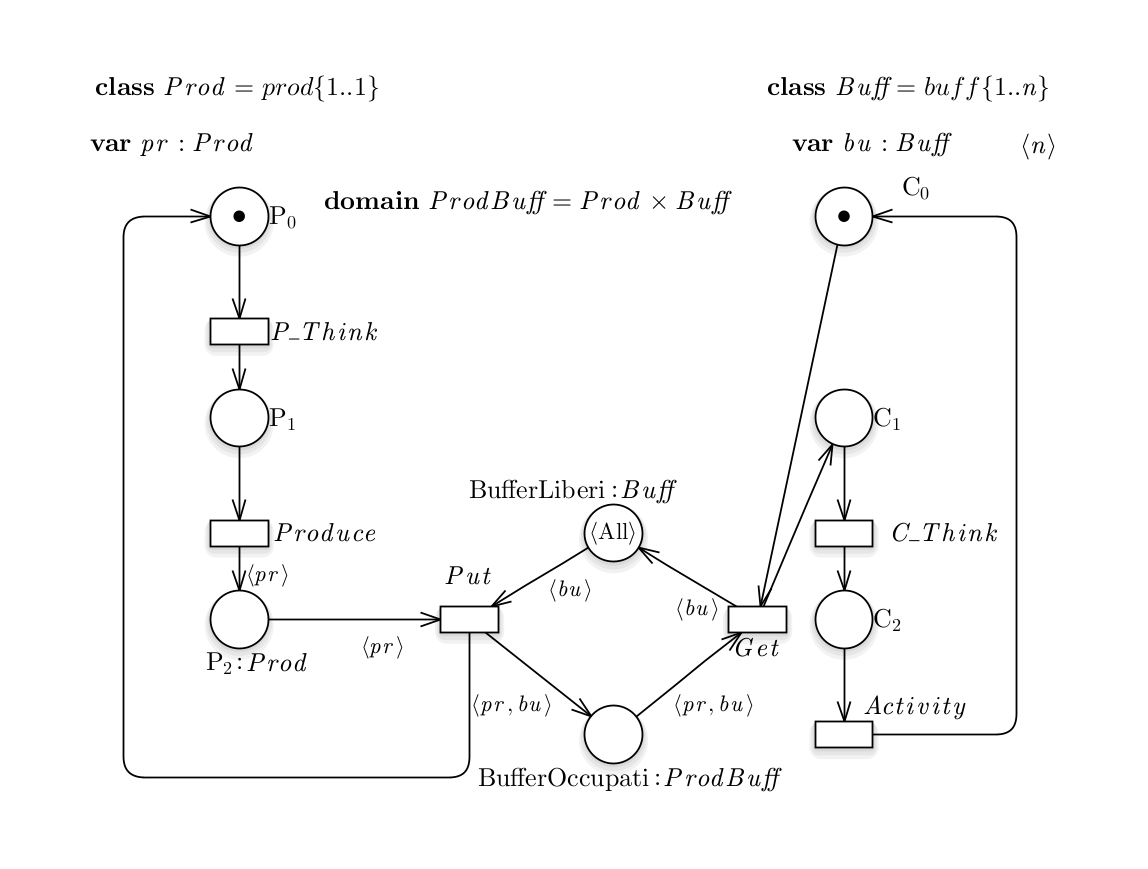
\includegraphics[scale=0.4]{Setting1def-2.png}
\end{figure}
\subsection{Modelling Convenience}
L'implementazione del Primo Setting ha richiesto in particolar modo di evidenziare come, nella rete di Petri colorata, gestire il \textit{Buffer} definendo il prodotto cartesiano tra Produttore e Buffer in maniera tale da evidenziale che ciascu token nel posto \textit{BufferLiberi} può essere associato a un solo Produttore mediante la transizione \textit{Put}.
\subsection{Solution Convenience}
Confronto del numeri di stati ottenuto tra il RG e il SRG con N che indica il numero di Token nel posto BufferLiberi:
\\\\
\begin{tabular}{|p{3cm}||p{3cm}|p{3cm}|}
\hline
N & RG & SRG\\
\hline
1&18&18\\
2&36&27\\
3&72&36\\
\hline
\end{tabular}
\\\\Dal confronto si osserva che il Symbolic Reachability Graph presenta un numero inferiore di stati rispetto a quelli ottenuti dal Colored Reachability Graph nel caso in cui il Buffer abbia un numero di token iniziali nel posto \textit{BufferLiberi} maggiore di 1, mentre nel caso in cui ci sia un solo token il numero è identico. 
\clearpage
\section{Secondo Setting}
Nel Secondo Setting è richiesta la Rete di Petri Colorata per lo schema Produttore - Consumatore in cui sono presenti: 1 Produttore, 2 Consumatori e Buffer a N posizioni. 
A differenza del Setting 1, si aggiungere un ulteriore Consumatore mediante la class domain \textit{Cons} in cui la costante C, che definisce il numero di Consumatori, è impostata a 2 modificando pertanto la marcatura iniziale del posto \textit{C0}. Inoltre è stato richiesto di associare i posti e gli archi rimanenti della struttura del Consumatore associandoli rispettivamente i posti alla color domain \textit{Cons} e le transizioni alla variabile \textit{co}.
\begin{figure}[h] 
\centering
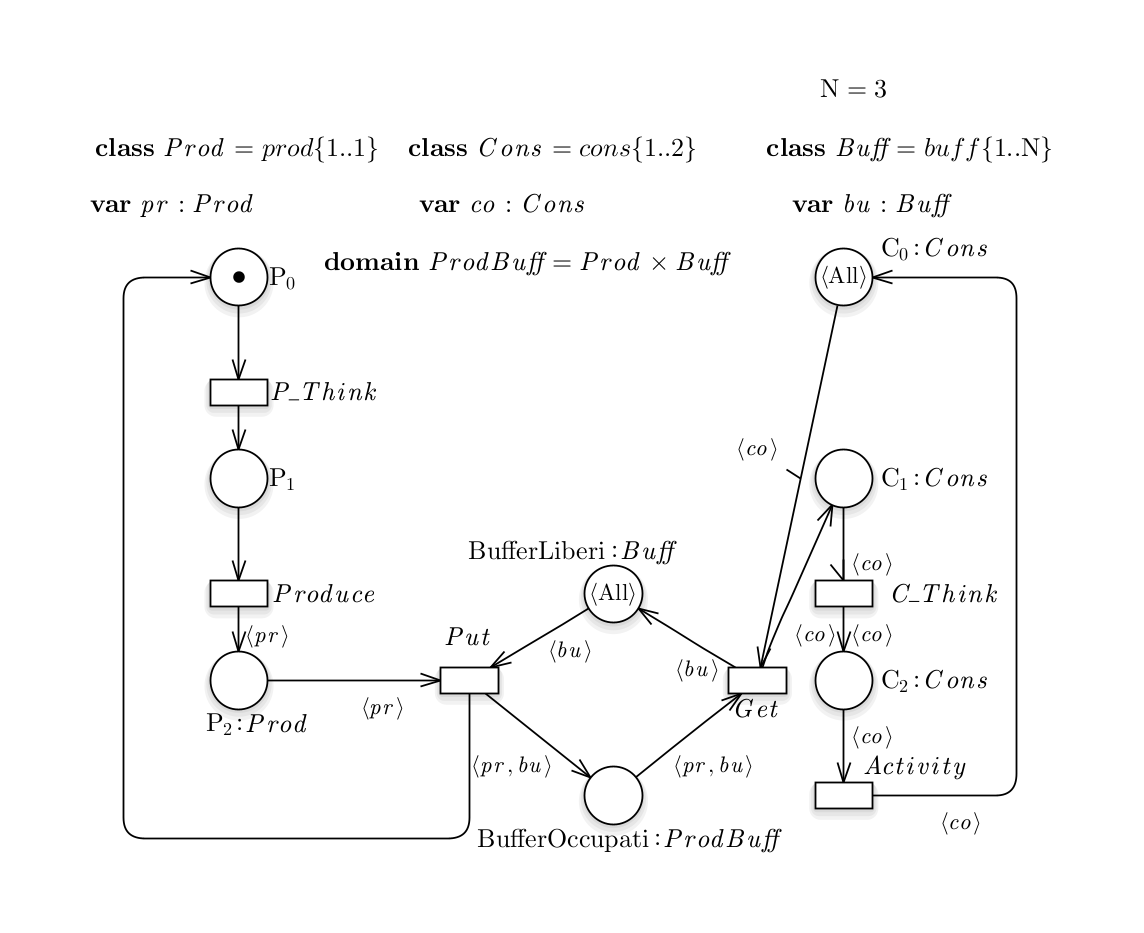
\includegraphics[scale=0.4]{Setting2def.png}
\end{figure}
\subsection{Modelling Convenience}
In questo Setting, la difficoltà principale è stata la modifica nella struttura del Consumatore in maniera tale da associare i posti alla color domain \textit{Cons} e le transizioni alla variabile \textit{co}.
\subsection{Solution Convenience}
Confronto del numeri di stati ottenuto tra il RG e il SRG con N che indica il numero di Token nel posto BufferLiberi:
\\\\
\begin{tabular}{|p{3cm}||p{3cm}|p{3cm}|}
\hline
N & RG & SRG\\
\hline
1&54&36\\
2&108&54\\
3&216&72\\
\hline
\end{tabular}\\\\Dal confronto si osserva che il Symbolic Reachability Graph presenta un numero inferiore di stati rispetto a quelli ottenuti dal Colored Reachability Graph in tutti i casi analizzati. 
\clearpage
\section{Terzo Setting}
Nel Terzo Setting è richiesta l'implementazione di una Rete di Petri Colorata per il problema Produttore - Consumatore in cui sono presenti: P Produttori, C consumatori e il Buffer a N posizioni.
\\Pertanto si è deciso di modificare anche per la rete del Produttore, come avvenuto nel Setting 2 per il Consumatore, associando posti e transizioni rispettivamente alla color domain \textit{Prod} e la variabile \textit{pr}.
La struttura della rete rimane varia mediante una modifica nei posti iniziali, sia per il Produttore sia per il Consumatore, associando i posti iniziali alla color domain rispettiva \textit{Prod} e \textit{Cons}. Analagomente al Setting 2 per la struttura del Consumatore, anche per il Produttore è stato richiesto di modificare la restante parte della rete pertanto si associa alle transizioni del produttore \textit{pr}.

\begin{figure}[h] 
\centering
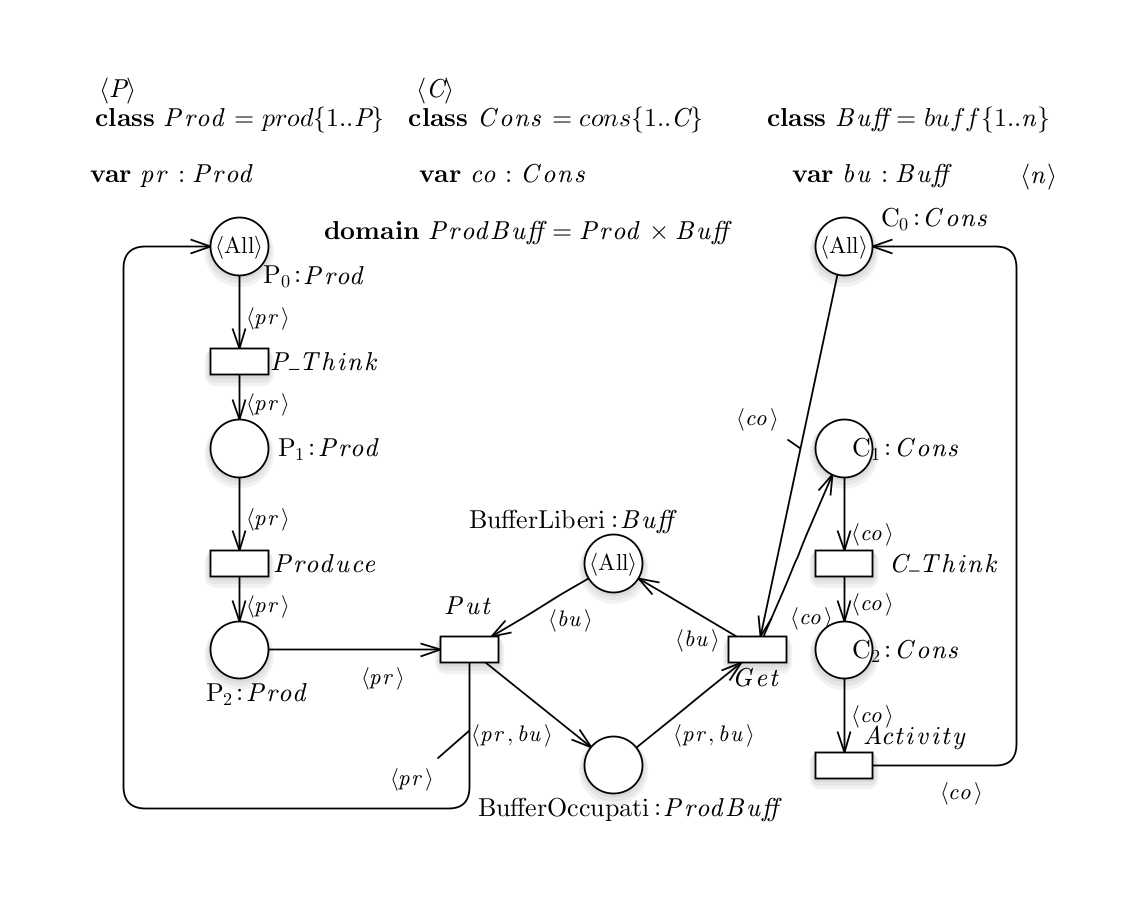
\includegraphics[scale=0.4]{WN-Setting3-Marcatura.png}
\end{figure}
\clearpage
\subsection{Modelling Convenience}
In questo Setting, la difficoltà principale è stata la modifica nella struttura del Produttore in maniera tale da associare i posti alla color domain \textit{Prod} e le transizioni alla variabile \textit{pr}.
\subsection{Solution Convenience}
Confronto del numeri di stati ottenuto tra il RG e il SRG definendo 2 Produttori e 2 Consumatori e con N che indica il numero di Token nel posto BufferLiberi:
\\\\
\begin{tabular}{|p{3cm}||p{3cm}|p{3cm}|}
\hline
N & RG & SRG\\
\hline
1&243&90\\
2&729&180\\
3&2187&288\\
\hline
\end{tabular}
\\\\Dal confronto si osserva che il Symbolic Reachability Graph presenta un numero inferiore di stati rispetto a quelli ottenuti dal Colored Reachability Graph in tutti i casi analizzati. 
\end{document}